
\textbf{A.1 Humans have a robust visuomotor control system that supports walking in complex environments.}

Closed loop system:

[stepping influences seeing] Biomechanics of walking constrains visual behavior 
- we look 2-5 steps ahead (Jon lab stuff, patla stuff, Jon/Mary/Kate stuff)

[seeing influences stepping] 
Kuo: incorporate upcoming obstacles to maximize energetic efficiency

- We don't have a model human walkers. And frankly we don't even have the right dataset.  Most datasets aren't egocentric.  The datasets that are do not include complete body pose information that allows us to understand the relationship between visual perception and action.

The large datasets that are being generated only have eye movements and
world content: ego 4d and other long list of stuff. An old idea in
cognitive science and visual perception that has gained traction in the
ML community via reinforcement learning approaches is that the ability
to take action and adjust your own input influences learning. We need
datasets with stored actions to make this happen\ldots{}\newline


\noindent \textbf{A.2 Visual search patterns are efficient and task-dependent}

\noindent There is strong evidence from investigations into visual search for targets within natural scene statistics that search patterns are highly fixation-efficient and subsequent eye movements are made to maximize the probability of finding the target \cite{najemnik_optimal_2005}. Additionally, there is a body of research which demonstrates that visual search is highly task-dependent \cite{jovancevic-misic2009, tong2017, zhang2018, hayhoe2005, tatler2011, rothkopf2016}. This research demonstrates that the visual system works to provide information relevant to the goals of the perceiver, such that eye movements are efficiently made to serve the current task demands and reduce uncertainty \cite{Matthis2018}. 

EXAMPLE FROM MORE TYPICAL VISUAL SEARCH LITERATURE

What information is most relevant for the task of locomotion?

Recently, [WE] conducted the first investigation into eye movements made while traversing natural outdoor terrains of varying difficulty \cite{Matthis2018,hayhoe2018} (Fig. 1). Examination of this data demonstrates that eye movements made during visual search are likely influenced by the biomechanical constraints of the locomotor system: walkers fixate where they want to step as opposed to visually salient terrain. Critically, this observation – that the proprioceptive information of biomechanics might influence visual search – is substantiated by recent work in biomechanics.

Examinations of bipedal biomechanics consistently demonstrate that human locomotion is energetically efficient\cite{Kuo2002,Donelan2002}. Recently, researchers have shown that the humans are constantly adapting their gait to maintain energetically optimal movements even seconds after perturbation \cite{selinger2015}. This, combined with evidence that humans can readily perceive energetically efficient\cite{warren1984} or optimal body movements \cite{weast-knapp2019}, suggests that the visual system must be seeking information which allows for energetically efficient foot placements.

ANOTHER PARAGRAPH HERE


\textbf{A.3 } 


\textbf{A.4 Summary of significance.} 

overall scientific premis of this proposal is bolstered by past research showing that...

This proposal is significant because it is designed to ...


  Furthermore, this gap restricts our understanding of how the visuo-locomotor system might be affected by aging and disease (e.g., retinal CITE, motor CITE).  



\begin{itemize}
\item
  Established the general patterns of visuomotor control, but now we
  need to:

  \begin{itemize}
  \item
    1. Leverage improved processes for collecting integrated visuomotor
    datasets to collect more precise, expanded datasets.
  \item
    2. Develop laboratory protocols that allow for the
  \end{itemize}
\end{itemize}
that allow for the

\begin{figure}[h]
\centering
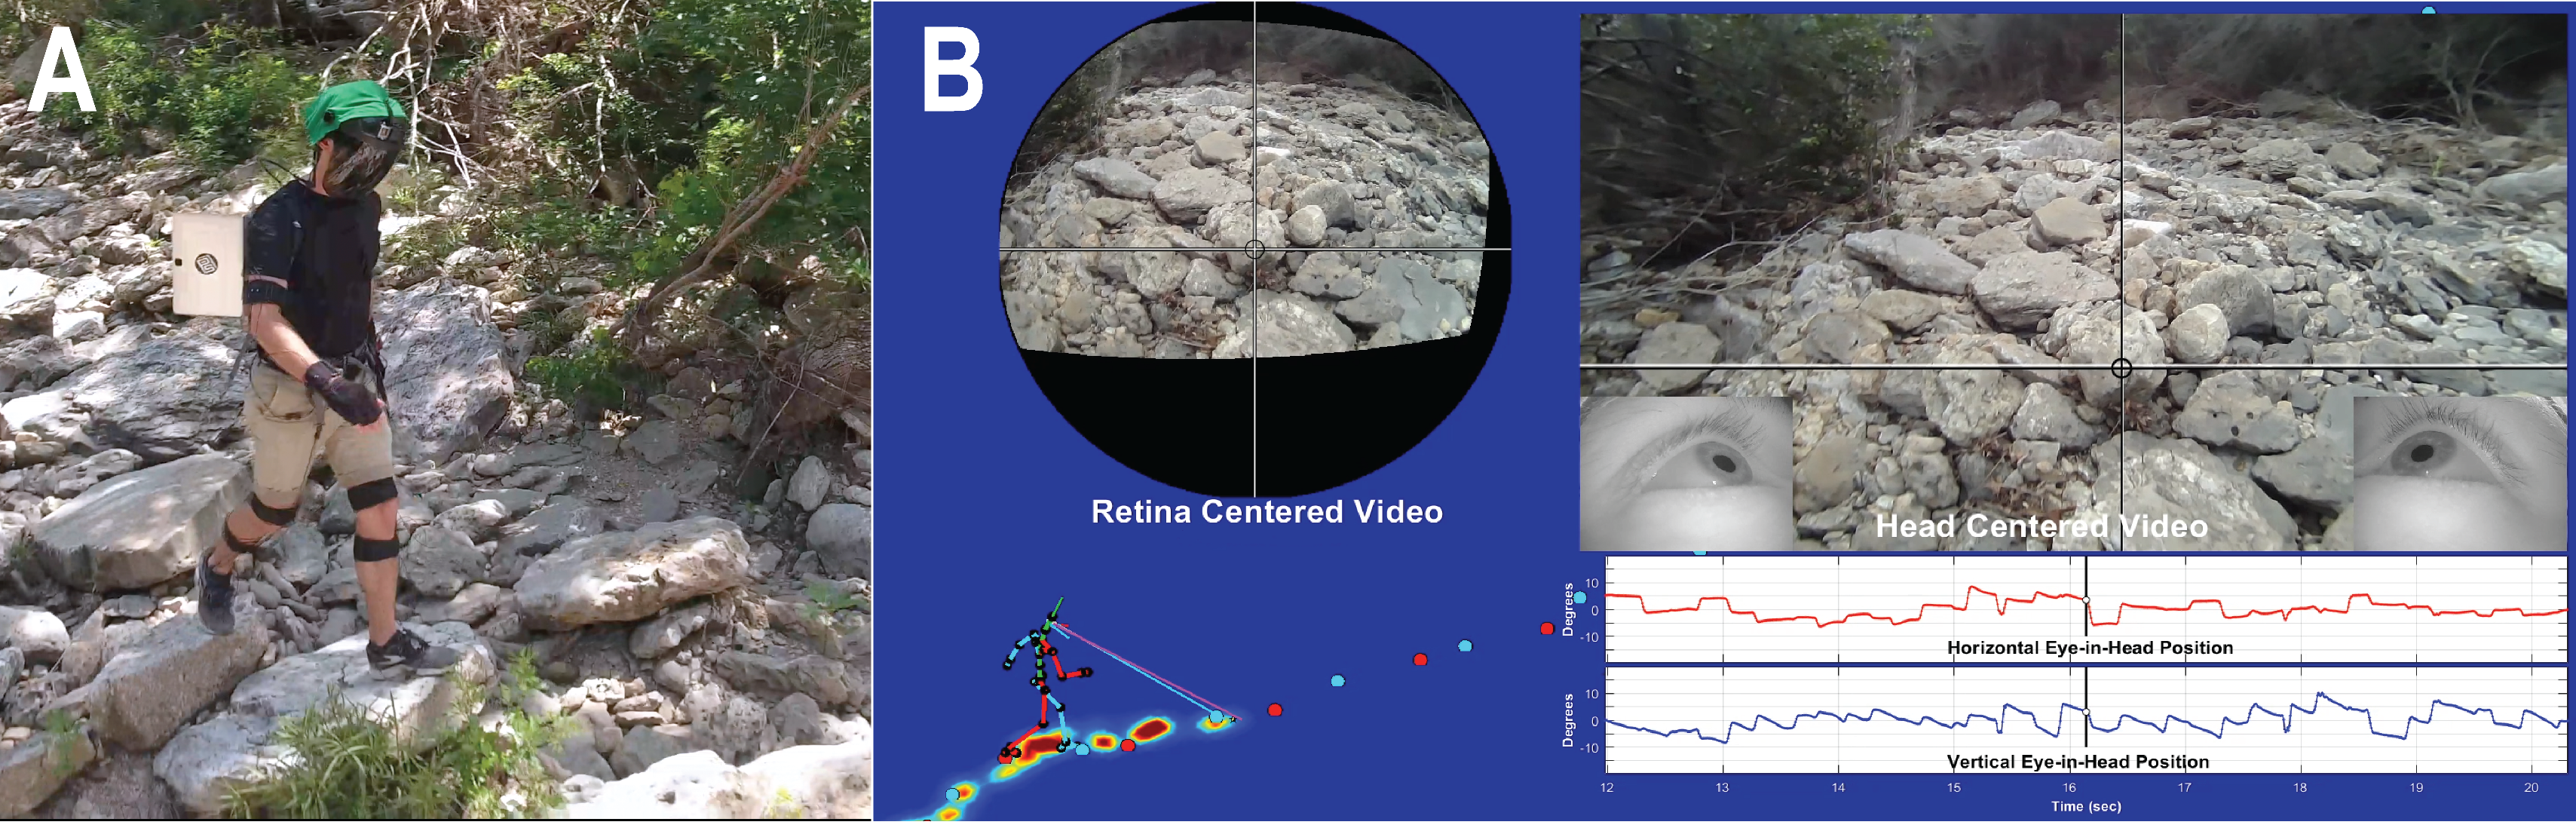
\includegraphics[width=\textwidth]{document/figures/Figure-1-outdoor-walking.pdf}
\caption{\textbf{Outdoor measurements of the visuo-locomotor system.} A. ?? B. ??}
\end{figure}
